\addcontentsline{toc}{section}{Supplementary Material}

\section{Limitations}
Our analysis is conducted on a single benchmark domain (SLR-Bench), which frames inductive reasoning through logic programming over train classification tasks. While the shortcut behaviors we identify are systematic and reproducible, the extent to which they generalize to other reasoning domains (e.g., mathematical, causal, or abductive reasoning) remains an open question. Furthermore, our evaluation of frontier models (GPT-5 family) is limited to black-box access, preventing direct inspection of reasoning traces or internal representations. IPT detects shortcuts through behavioral invariance testing, but cannot distinguish whether shortcut strategies are explicitly represented in the model's reasoning process or emerge implicitly from output distributions. Finally, our controlled training experiment uses a 7B-parameter model due to computational constraints; whether the observed training dynamics scale identically to larger model sizes warrants further investigation.




\section{Detailed Shortcut Analysis} \label{app:sec:shortcut_analysis}
A detailed overview of the entire evaluation is outlined in \autoref{tab:shortcut_overview}, along with aggregated trends in \autoref{fig:shortcut_trends}. The benchmark consists of tasks across four complexity tiers, each consisting of 5 complexity levels: \textit{Basic} (level 1-5), \textit{Easy} (level 6-10), \textit{Medium} (level 11-15), and \textit{Hard} (level 16-20). Each model performs a single inference pass per task, and the resulting hypothesis is evaluated under both extensional and isomorphic verification.

\autoref{tab:shortcut_overview} reports tier-wise accuracy and the number of reward shortcuts ($N_S$). Accuracy is defined as the percentage of tasks solved under isomorphic verification, requiring genuine rule induction. The shortcut count $N_S$ measures the number of tasks (out of $250$ per tier) where a hypothesis satisfies extensional verification but fails under isomorphic verification. In addition, \autoref{fig:shortcut_trends} reports the \textit{shortcut rate}, defined as the ratio of shortcuts to the total number of tasks, i.e.,  $\text{shortcut rate} = N_S / N_{\text{tasks}}$.


\textbf{Model-scale - shortcut trend.}
\autoref{tab:shortcut_overview} reveals substantial variation across model scales. Larger models such as \symbols{gpt-5} exhibit relatively few shortcuts, whereas smaller models (e.g., \symbols{gpt-5-mini-high}, \symbols{gpt-5-nano}) show significantly higher shortcut counts. Notably, \symbols{gpt-5-nano} exhibits extreme shortcut reliance in higher complexity tiers. This suggests that smaller models possess a weaker internal representation of the task objective, making them more susceptible to derailing into shortcut strategies rather than pursuing genuine rule induction. Larger models, by contrast, appear to maintain a more robust understanding of the underlying reasoning structure, resorting to shortcuts primarily as a deliberate fallback when task complexity exceeds their inductive capacity. Then, extensional enumeration offers a viable strategy to game the verifier rather than returning no reward at all.


\textbf{RLVR optimization pressure - shortcut trend.}
\autoref{tab:shortcut_overview} shows that \symbols{olmo-3-32b} exhibits no shortcut behavior. In contrast, \symbols{olmo-3.1} trained under the same setup but with extended RLVR optimization begins to exhibit shortcuts. This indicates that shortcut strategies are not merely present, but are actively \emph{discovered and reinforced} through optimization. As training progresses, RL increasingly amplifies behaviors that maximize the reward signal. When the verifier is imperfect, this creates an optimization landscape in which shortcut strategies can yield high reward without requiring genuine reasoning. Over time, these strategies become more prominent, suggesting that continued optimization pressure can shift the model toward policies that are better at exploiting the verifier rather than solving the underlying task.


\textbf{Task complexity - shortcut trend.}
Across models, shortcut behavior is heavily concentrated in the \textit{Medium} and \textit{Hard} tiers. As shown in \autoref{fig:shortcut_trends} (left), shortcut rates remain low for \textit{Basic} tasks, but increase sharply with complexity. This suggests a qualitative shift in strategy: when tasks are simple, models can satisfy the objective via genuine rule induction; as complexity increases and induction becomes more difficult, optimization pressure favors alternative strategies that achieve high reward at lower cost. Shortcut behavior thus appears not as a random failure, but as a systematic fallback when induction becomes computationally or search-wise expensive.

\textbf{Reasoning effort - shortcut trend.}
\autoref{fig:shortcut_trends} (right) shows that increasing inference-time compute leads to higher shortcut rates. For the \symbols{gpt-5-mini} family, scaling reasoning effort from low to high results in a monotonic increase in shortcut prevalence. This indicates that additional compute is not inherently aligned with better reasoning. Instead, it expands the search over possible strategies, including those that exploit weaknesses in the verifier. In this sense, more compute amplifies the model’s ability to discover reward-maximizing behaviors—whether or not they correspond to the intended reasoning process.




% \begin{table*}[t]
% \centering
% \resizebox{\textwidth}{!}{
% \begin{tabular}{lccrrrrr|rrrrr|rrr}
% \toprule
% & \multicolumn{2}{c}{\textit{Reasoning RL via}} 
% & \multicolumn{5}{c}{\textit{Logical Reasoning Accuracy (\%)}} 
% & \multicolumn{5}{c}{\textit{\# Reward Shortcuts ($N=250$)}} 
% & \multicolumn{3}{c}{\textit{Efficiency \& Cost}} \\
% \cmidrule(lr){2-3} \cmidrule(lr){4-8} \cmidrule(lr){9-13} \cmidrule(lr){14-16}
% Model & AI-Feedback & RLVR 
% & Basic & Easy & Med. & Hard & Avg 
% & Basic & Easy & Med. & Hard & $\sum$ 
% & Tokens & Costs & Syntax \\
% \midrule

% \rowcolor{reasoningllm!50} gpt-5 & (\cmark) & (\cmark) 
% & 100 & 100 & 77 & 50 & 82 
% & 0 & 0 & 3 & 1 & 4 
% & -- & -- & -- \\

% \rowcolor{reasoningllm!50} gpt-5-mini-high & (\cmark) & (\cmark) 
% & 100 & 100 & 77 & 44 & 80 
% & 0 & 1 & 24 & 59 & 84 
% & -- & -- & -- \\

% \rowcolor{reasoningllm!50} gpt-5-mini & (\cmark) & (\cmark) 
% & 100 & 99 & 50 & 23 & 68 
% & 0 & 0 & 14 & 18 & 32 
% & -- & -- & -- \\

% \rowcolor{reasoningllm!50} gpt-5-mini-low & (\cmark) & (\cmark) 
% & 100 & 85 & 26 & 8 & 55 
% & 0 & 0 & 0 & 0 & 0 
% & -- & -- & -- \\

% \rowcolor{reasoningllm!50} gpt-5-nano & (\cmark) & (\cmark) 
% & 100 & 75 & 12 & 3 & 47 
% & 0 & 37 & 147 & 184 & 368 
% & -- & -- & -- \\

% \midrule

% \rowcolor{reasoningllm!50} Olmo-3.1-32B & \cmark & \cmark 
% & 91 & 60 & 10 & 2 & 41 
% & 2 & 0 & 3 & 5 & 10 
% & -- & -- & -- \\

% \rowcolor{reasoningllm!50} Olmo-3-32B & \cmark & \cmark 
% & 84 & 53 & 9 & 2 & 37 
% & 0 & 0 & 0 & 0 & 0 
% & -- & -- & -- \\

% \rowcolor{reasoningllm!50} Olmo-3-7B & \cmark & \cmark 
% & 41 & 26 & 2 & 0 & 17 
% & 0 & 0 & 0 & 0 & 0 
% & -- & -- & -- \\

% \midrule

% \rowcolor{reasoningllm!50} Ministral-3-14B & \cmark & \xmark 
% & 82 & 58 & 13 & 5 & 40 
% & 0 & 0 & 0 & 0 & 0 
% & -- & -- & -- \\

% \rowcolor{reasoningllm!50} Ministral-3-8B & \cmark & \xmark 
% & 89 & 57 & 10 & 2 & 39 
% & 0 & 0 & 0 & 0 & 0 
% & -- & -- & -- \\

% \rowcolor{reasoningllm!50} Ministral-3-3B & \cmark & \xmark 
% & 78 & 43 & 6 & 2 & 32 
% & 0 & 0 & 0 & 0 & 0 
% & -- & -- & -- \\

% \midrule

% \rowcolor{basellm!50} gpt-4.5-preview & (\xmark) & (\xmark) 
% & 94 & 47 & 5 & 1 & 37 
% & 0 & 0 & 0 & 0 & 0 
% & -- & -- & -- \\

% \rowcolor{basellm!50} gpt-4o & (\xmark) & (\xmark) 
% & 93 & 29 & 2 & 0 & 31 
% & 0 & 0 & 0 & 0 & 0 
% & -- & -- & -- \\

% \rowcolor{basellm!50} gpt-4-turbo & (\xmark) & (\xmark) 
% & 89 & 18 & 2 & 0 & 27 
% & 0 & 0 & 0 & 0 & 0 
% & -- & -- & -- \\

% \bottomrule
% \multicolumn{16}{l}{\small \textit{Note:} Tok. = average reasoning tokens. Acc/1k Tok. = efficiency. \$ / Task = estimated inference cost. Parenthesized values (\cmark/\xmark) indicate presumed training methodology.}
% \end{tabular}
% }
% \caption{{LLM shortcut behavior.} Comparison of logical reasoning accuracy, reward shortcuts, and efficiency/cost.}
% \label{tab:shortcut_overview}
% \end{table*}

\begin{table*}[t]
\centering
\resizebox{\textwidth}{!}{
\begin{tabular}{lcc | rrrr | rrrr | rrr}
\toprule
& \multicolumn{2}{c}{\textit{Reasoning RL}} 
& \multicolumn{4}{c}{\textit{Reasoning Accuracy (\%)}} 
& \multicolumn{4}{c}{\textit{\# Shortcuts ($N = 250$)}} 
& \multicolumn{3}{c}{\textit{Efficiency \& Cost}} \\
\cmidrule(lr){2-3} \cmidrule(lr){4-7} \cmidrule(lr){8-11} \cmidrule(lr){12-14}
Model & Judge & RLVR
& Basic & Easy & Med. & Hard 
& Basic & Easy & Med. & Hard 
& Syntax & Tokens & USD \\
\midrule

\rowcolor{reasoningllm!50} Gpt-5 & (\cmark) & (\cmark)
& 100 & 100 & 77 & 50 & 0 & 0 & 3 & 1 & 100 & 9.4M & 103.13 \\

\rowcolor{reasoningllm!50} Gpt-5 Mini\textsuperscript{H} & (\cmark) & (\cmark)
& 100 & 100 & 74 & 44 & 0 & 1 & 23 & 59 & 93 & 13.1M & 27.98 \\

\rowcolor{reasoningllm!50} Gpt-5 Mini\textsuperscript{M} & (\cmark) & (\cmark)
& 100 & 98 & 50 & 23 & 0 & 0 & 14 & 18 & 98 & 4.9M & 11.54 \\

% \rowcolor{reasoningllm!50} Gpt-5-Mini\textsuperscript{M}(no-cheat) & (\cmark) & (\cmark)  & 100 & 98 & 52 & 24 & 0 & 0 & 8 & 12 & 98 & 5.1M & 11.87 \\


\rowcolor{reasoningllm!50} Gpt-5 Mini\textsuperscript{L} & (\cmark) & (\cmark)
& 100 & 85 & 26 & 8 & 0 & 0 & 0 & 0 & 98 & 1.2M & 4.07 \\

\rowcolor{reasoningllm!50} Gpt-5 Nano & (\cmark) & (\cmark)
& 99 & 74 & 12 & 3 & 0 & 37 & 147 & 184 & 99 & 6.2M & 2.81 \\

\midrule

\rowcolor{reasoningllm!50} OLMo-3.1 32B & \cmark & \cmark
& 81 & 60 & 11 & 2 & 2 & 1 & 3 & 7 & 98 & 14.6M & -- \\

\rowcolor{reasoningllm!50} OLMo-3 32B & \cmark & \cmark
& 99 & 68 & 11 & 2 & 0 & 0 & 0 & 0 & 98 & 16.0M & 9.04 \\

\rowcolor{reasoningllm!50} OLMo-3 7B & \cmark & \cmark
& 30 & 15 & 1 & 0 & 0 & 0 & 0 & 0 & 95 & 17.8M & -- \\

\midrule

\rowcolor{reasoningllm!50} Ministral-3 14B & \cmark & \xmark
& 90 & 74 & 17 & 7 & 0 & 0 & 0 & 0 & 50 & 2.7M & 0.82 \\

\rowcolor{reasoningllm!50} Ministral-3 8B & \cmark & \xmark
& 90 & 63 & 10 & 2 & 0 & 0 & 0 & 0 & 47 & 1.5M & 0.43 \\

\rowcolor{reasoningllm!50} Ministral-3 3B & \cmark & \xmark
& 79 & 47 & 7 & 2 & 0 & 0 & 0 & 0 & 61 & 3.5M & 0.77 \\

\midrule

\rowcolor{basellm!50} Gpt-5 (chat) & (\xmark) & (\xmark)
& 100 & 91 & 34 & 14 & 0 & 0 & 0 & 0 & 100 & 2.7M & 36.04 \\

\rowcolor{basellm!50} Gpt-4.5 Preview & (\xmark) & (\xmark)
& 96 & 61 & 6 & 2 & 0 & 0 & 0 & 0 & 100 & 0.4M & 576.40 \\

\rowcolor{basellm!50} Gpt-4o & (\xmark) & (\xmark)
& 95 & 31 & 2 & 1 & 0 & 0 & 0 & 0 & 100 & 0.3M & 20.03 \\

\rowcolor{basellm!50} Gpt-4o-mini & (\xmark) & (\xmark)
& 92 & 18 & 0 & 0 & 0 & 0 & 0 & 0 & 100 & 0.4M & 1.26 \\

\rowcolor{basellm!50} Gpt-4 Turbo & (\xmark) & (\xmark)
& 93 & 20 & 2 & 0 & 0 & 0 & 0 & 0 & 100 & 0.4M & 81.30 \\

\bottomrule
\multicolumn{14}{l}{\small Parenthesized values (\cmark/\xmark) indicate presumed training methodology. Reasoning effort: \textsuperscript{L}: Low, \textsuperscript{M}: Medium, \textsuperscript{H}: High, --: No pricing information available.}
\end{tabular}
}
\caption{Comparison of logical reasoning accuracy, reward shortcuts, and efficiency across models.}
\label{tab:shortcut_overview}
\end{table*}


\begin{figure*}[t]
    \centering
    \begin{subfigure}[t]{.47\textwidth}
        \centering
        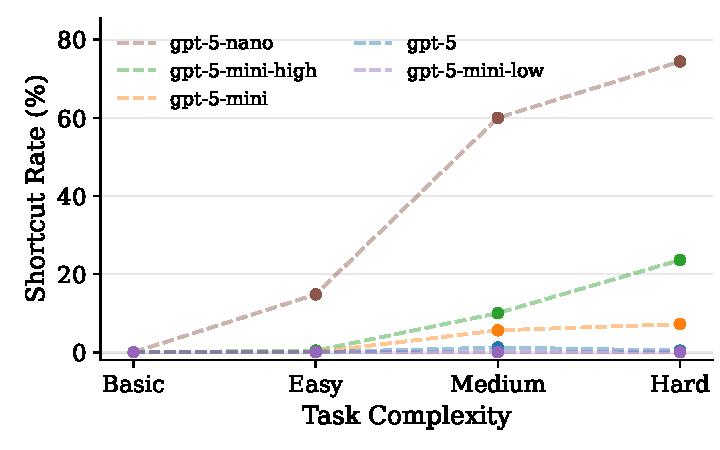
\includegraphics[width=\textwidth]{figs/paper_complexity_short_pressure.pdf}
        \caption{As models face more complex reasoning tasks, they increasingly resort to shortcut behaviours.}
        \label{app:fig:complexity_trend}
    \end{subfigure}
    \hfill
    \begin{subfigure}[t]{.47\textwidth}
        \centering
        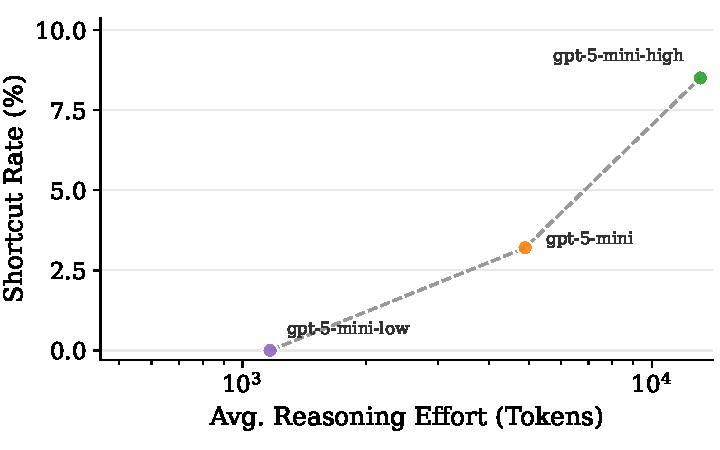
\includegraphics[width=\textwidth]{figs/paper_effort_short_pressure.pdf}
        \caption{As the reasoning effort of gpt-5-mini is scaled, the model increasingly resorts to shortcut behaviours.}
        \label{app:fig:gpt5_mini_trend}
    \end{subfigure}
    \caption{{Shortcut rate} ($\text{shortcuts}/\text{num tasks}$) as a function of task complexity and inference-time compute. Left: shortcut rate by complexity tiers. Right: shortcut rate by reasoning effort. Trends show that both increasing task difficulty and inference compute drive shortcut prevalence.}
    \label{fig:shortcut_trends}
\end{figure*}

\begin{figure*}[t]
    \centering
    \begin{subfigure}[t]{.47\textwidth}
        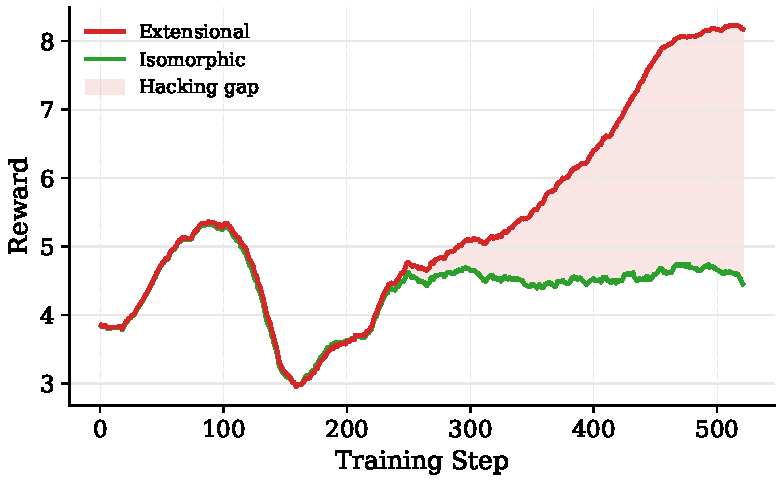
\includegraphics[width=\textwidth]{figs/training.pdf}
        \caption{Extensional RLVR: extensional reward diverges as the model learns to exploit the verifier.}
    \end{subfigure}
    \hfill
    \begin{subfigure}[t]{.47\textwidth}
        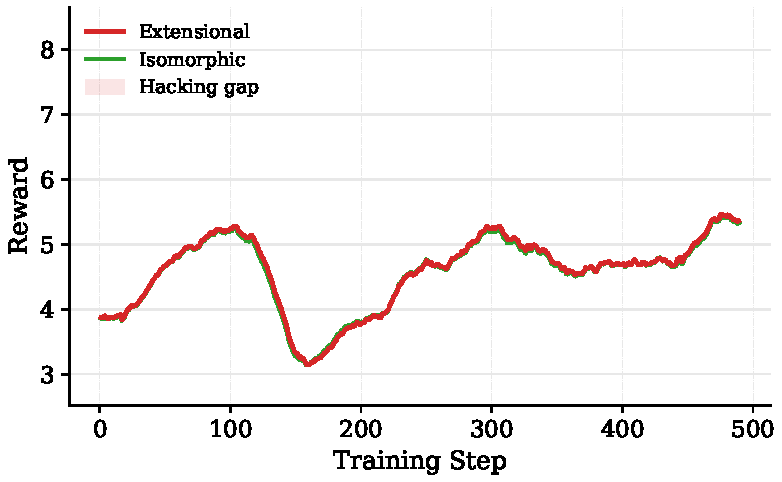
\includegraphics[width=\textwidth]{figs/training_iso_gap.pdf}
        \caption{Isomorphic RLVR: both rewards track each other throughout, with no hacking gap.}
    \end{subfigure}
    \caption{Training Olmo-3-7B-Think-DPO via extensional vs. isomorphic RLVR. The hacking gap (shaded) only emerges when the model is trained against an extensional verifier.}
    \label{fig:training_dynamics}
\end{figure*}
\section{RLVR under Isomorphic vs. Non-Isomorphic Reward}\label{app:sec:training}

To validate that the reward shortcuts observed in frontier models can be a consequence of RLVR optimization of extensional verifiers, we conduct a controlled training experiment on \benchmark. We train two variants of the same base model under identical conditions, differing only in the reward signal: one receives feedback from the \emph{extensional verifier}, the other from the \emph{isomorphic verifier}. 

To validate that the reward shortcuts observed in frontier models can arise from RLVR optimization against extensional verification, we conduct a controlled training experiment on \benchmark. We follow the default Olmo-3 RLVR setup (\texttt{Olmo-core} + \texttt{Open Instruct}) \cite{olmo2025olmo3} and finetune two variants of Olmo-3-7B-Think-DPO using \benchmark\cite{helff2025slr}. The two runs only differ in the reward signal: one receives feedback from the \emph{extensional verifier}, the other from the \emph{isomorphic verifier}. We train for about 500 steps per run using 64 H100 GPUs for about 48h.

\autoref{fig:training_dynamics} reports the extensional and isomorphic rewards throughout training. The maximum reward under the Olmo-3 RLVR setup is 10. In the extensional run, both rewards initially track each other; around step 250 they diverge sharply. The extensional reward continues to climb while the isomorphic reward plateaus, indicating that the model has discovered and exploited shortcut strategies that satisfy the extensional verifier without performing genuine rule induction. The shaded region (hacking gap, $r_{\text{ext}} - r_{\text{iso}}$) grows monotonically, reaching a gap of approximately 3.5 reward points after 500 steps. In the isomorphic run, the gap remains near zero throughout, confirming that training against the isomorphic verifier prevents shortcut behaviour. These results provide direct causal evidence that an imperfect extensional reward signal is sufficient to induce reward hacking, and that isomorphic verification removes this incentive.

